\documentclass[12pt,openright,oneside,a4paper,english,french,spanish]{abntex2}

\usepackage{cmap}
\usepackage{tikz}
\usepackage{lmodern}
\usepackage[T1]{fontenc}
\usepackage[utf8]{inputenc}
\usepackage{lastpage}
\usepackage{float}
\usepackage{indentfirst}
\usepackage{pdflscape}
\usepackage{color}
\usepackage{graphicx}
\usepackage{units}
\usepackage[brazilian,hyperpageref]{backref}
\usepackage[alf]{abntex2cite}
\usepackage{bold-extra}
\usepackage{eso-pic}
\usepackage{enumitem}

\graphicspath{{resource/}}
\DeclareGraphicsExtensions{.png,.jpg,.pdf}
\def\checkmark{\tikz\fill[scale=0.4](0,.35) -- (.25,0) -- (1,.7) -- (.25,.15) -- cycle;}

\newcommand{\curso}[1]{\def\imprimircurso{#1}}

\newcommand\BackgroundPic{
	\put(0,0){
		\parbox[b][\paperheight]{\paperwidth}{
			\vfill
			\centering
			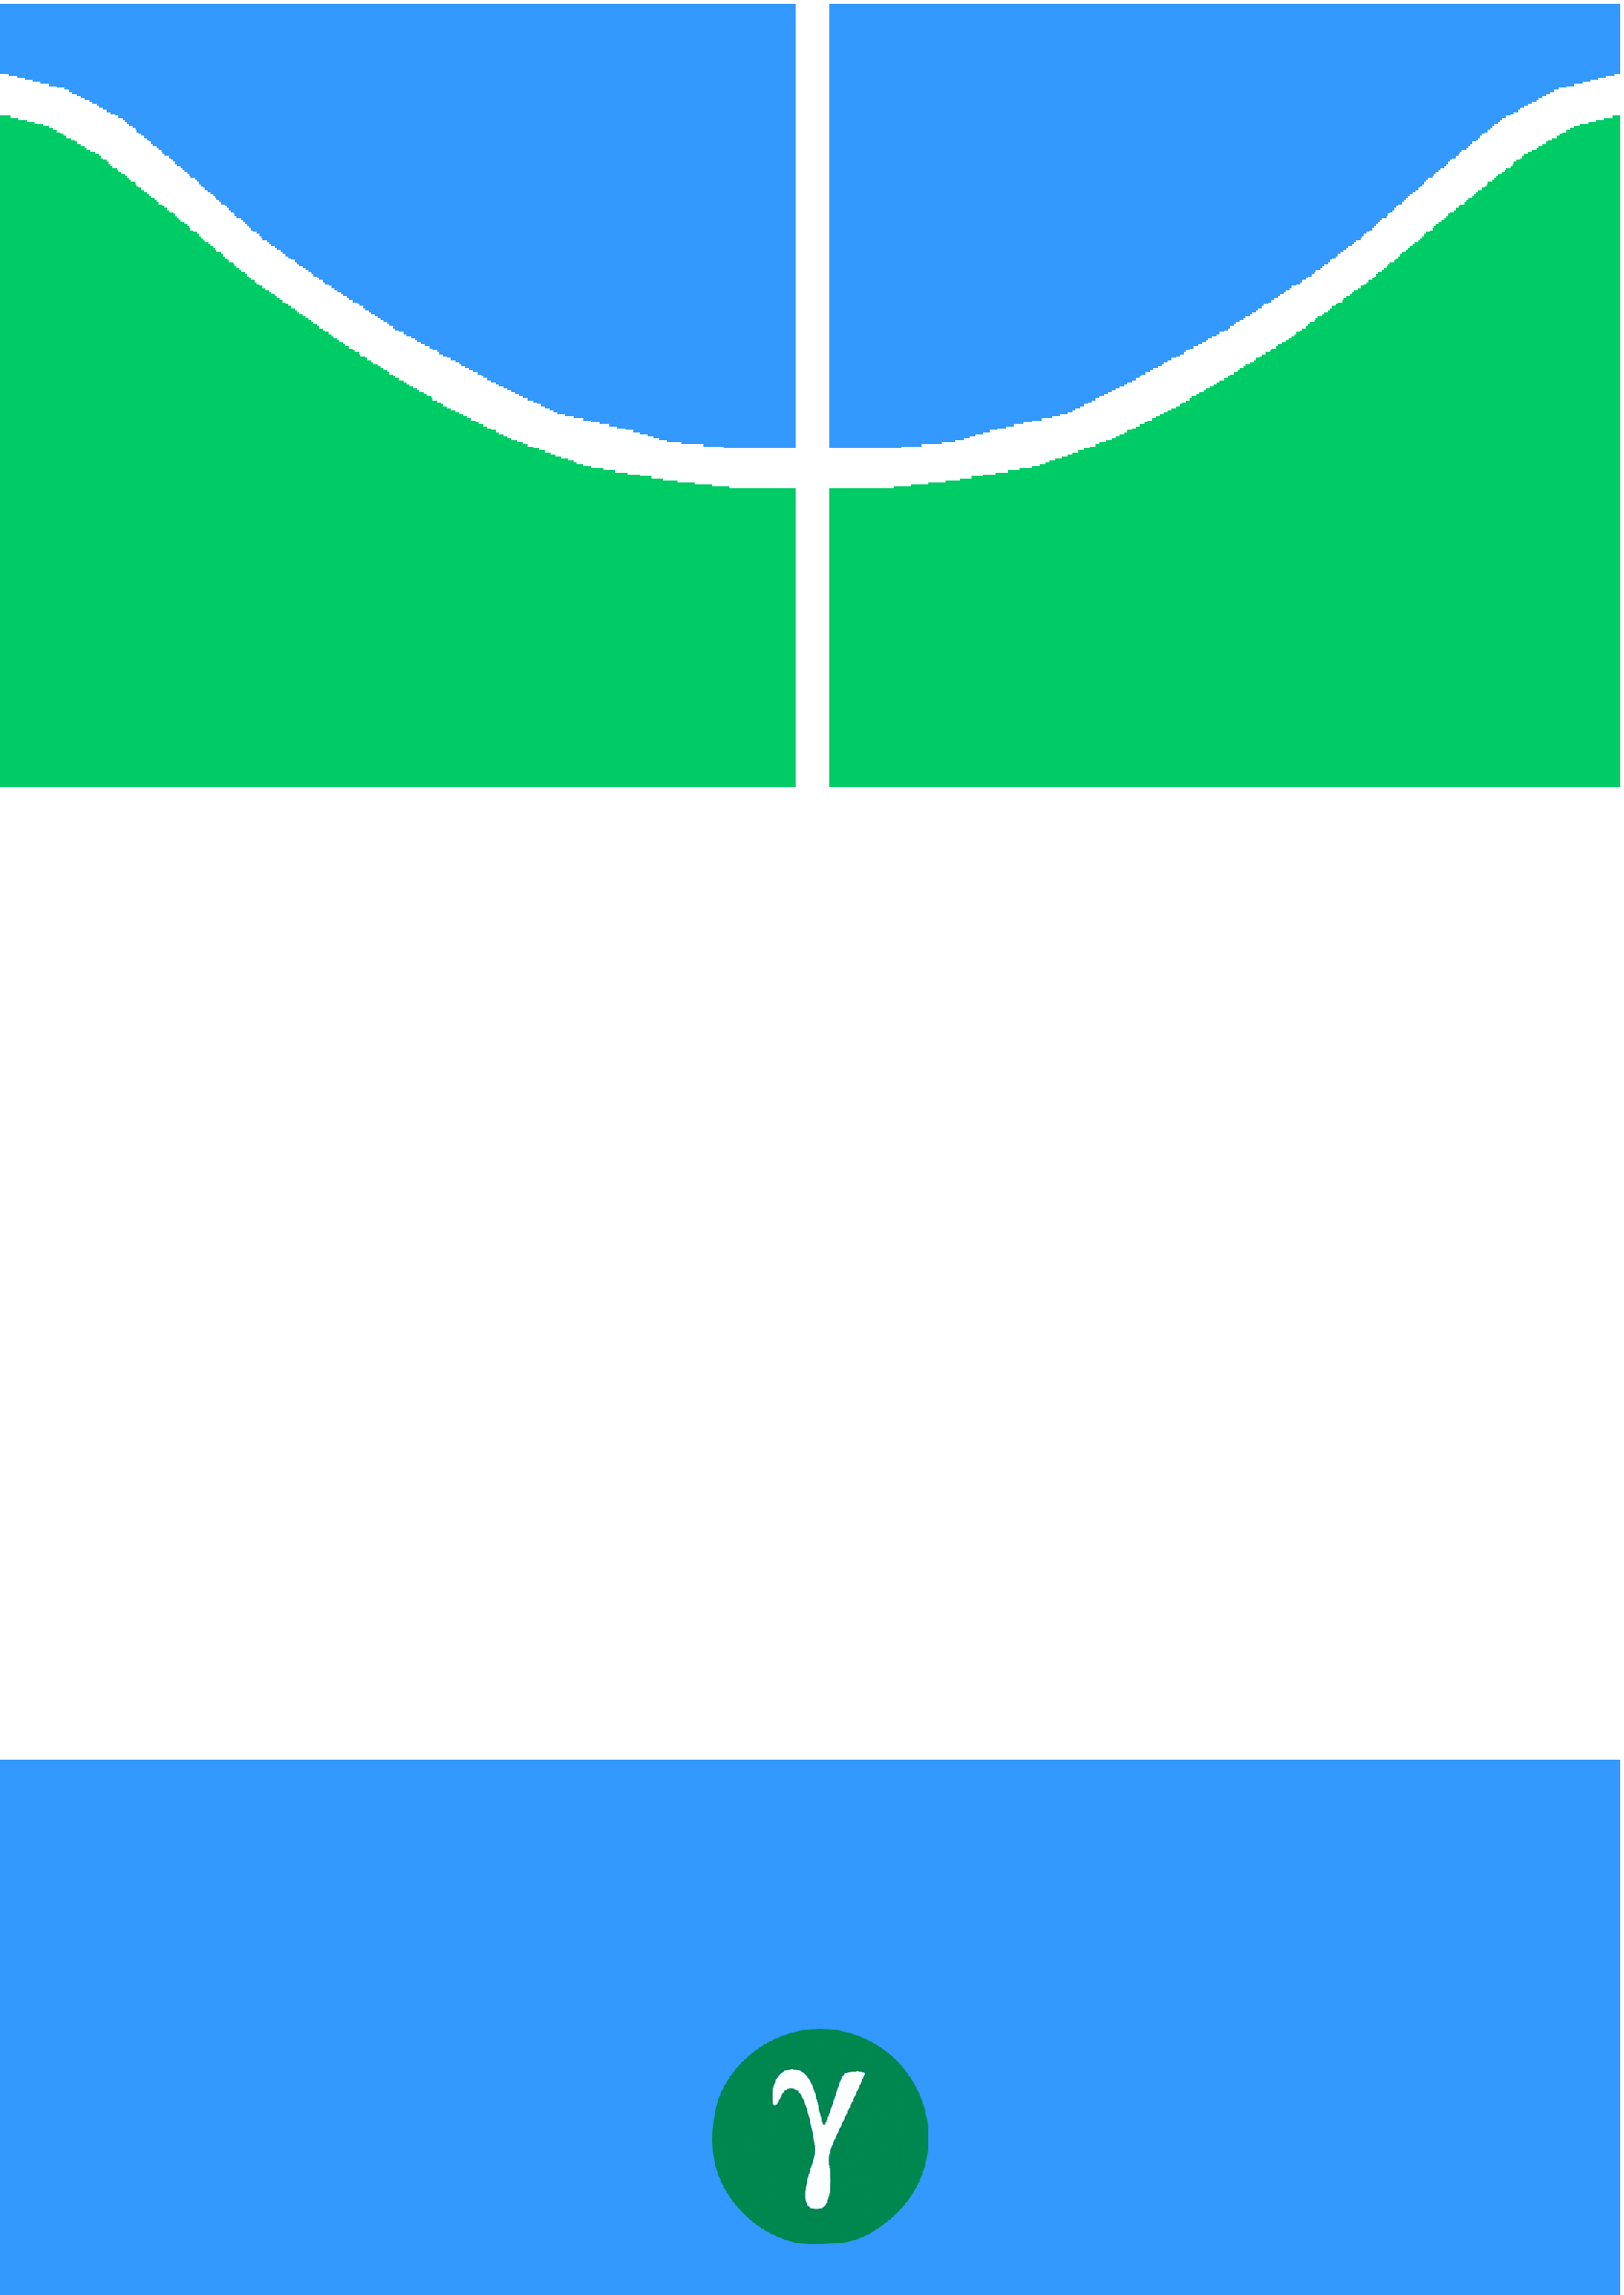
\includegraphics[width=\paperwidth,height=\paperheight,
				keepaspectratio]{capa}
			\vfill
		}
	}
}

\renewcommand{\imprimircapa}{
  \begin{capa}
    \center
	\AddToShipoutPicture*{\BackgroundPic}

    \vspace*{6.5cm}
	{\textbf{\large\imprimirinstituicao}}
	\par
	{\textbf{\large\imprimircurso}}

	\vspace*{1cm}

    {\ABNTEXchapterfont\bfseries\LARGE\imprimirtitulo}
    
	\begin{flushright}
    	\textbf{{\large{Grupo 75: \\ \imprimirautor}}}
		\par
    	\textbf{{\large{Orientador: \\ \imprimirorientador}}}
	\end{flushright}
		
    \vspace*{0.5cm}
    \textbf{{\large\imprimirlocal}}
    \par
    \textbf{{\large\imprimirdata}}
    
  \end{capa}
}

\renewcommand{\backrefpagesname}{Citado na(s) página(s):~}
\renewcommand{\backref}{}
\renewcommand*{\backrefalt}[4]{
	\ifcase #1 %
		Nenhuma citação no texto.%
	\or
		Citado na página #2.%
	\else
		Citado #1 vezes nas páginas #2.%
	\fi}%
% ---



% Dados Gerais
\autor{André Guedes, Caio Nardelli, Jonathan Moraes \\ Matheus Herlan, Matheus Oliveira e Pedro Tomioka}
\curso{Requisitos de Software - 201308 \\ Modelagem de Processos - 203921}

% Dados do trabalho
\titulo{Relatório 02 do Projeto de Melhoria CHAMEX}
\data{04 de Dezembro de 2014}

% Dados da orientacao
\orientador{George Marsicano Corrêa, MSc.}
\coorientador{}

\local{Brasília, DF}
\instituicao{
  Universidade de Brasília - UnB
  \par
  Faculdade UnB Gama - FGA
}
\tipotrabalho{Relatório de Engenharia de Software}
\preambulo{Trabalho submetido durante o curso de graduação em Engenharia de Software da Universidade de Brasília como requisito parcial para obtenção curricular da disciplina de Requisitos de \emph{Software} e Modelagem de Processos.}

\definecolor{black}{RGB}{0,0,0}
\makeatletter
\hypersetup{
		pdftitle={\@title}, 
		pdfauthor={\@author},
    	pdfsubject={\imprimirpreambulo},
		colorlinks=true,
    	linkcolor=black,
    	citecolor=black,
    	filecolor=magenta,
		urlcolor=black,
		bookmarksdepth=4
}
\makeatother
\setlength{\parindent}{1.3cm}
\setlength{\parskip}{0.2cm}  
\makeindex


\begin{document}

	\frontmatter
		\frenchspacing
		\imprimircapa
		\renewcommand{\imprimirorientadorRotulo}{ Orientador: }
		\imprimirfolhaderosto
		
		\newpage
\pdfbookmark[0]{\contentsname}{toc}
\tableofcontents*
\cleardoublepage

		\pdfbookmark[0]{\listfigurename}{lof}
\listoffigures*
\cleardoublepage
\pdfbookmark[0]{\listtablename}{lot}
\listoftables*
\cleardoublepage

		\begin{siglas}
	\item[Migue] X
\end{siglas}


	\textual

	\mainmatter

	%[RS]	Apresentar o entendimento do contexto de negócio (processo de negócio), no qual os requisitos serão identificados;
		\chapter[Contexto de Negócio]{Contexto de Negócio}
\label{chap:contexto}
	O grupo da disciplina de Requisitos de \emph{Software} (RS) ficou responsável por trabalhar, juntamente com o grupo da disciplina de Modelagem de Processos (MPR), soluções de \emph{software} para o contexto da empresa fictícia CHAMEX.
\\ \indent O objetivo da CHAMEX consiste em auxiliar pequenas e médias empresas privadas a melhorarem a qualidade de vida dos trabalhadores. Quanto mais disposição, vitalidade e alegria obtiver entre os trabalhadores, mais resultado positivo as empresas possuem.
\\ \indent Para concretização do suporte às empresas, a CHAMEX elaborou o Modelo de Avaliação (MOA). O principal objetivo desse modelo está atrelado à verificação do nível de satisfação e qualidade de vida dos funcionários de uma determinada organização. A CHAMEX apresenta um modelo de gestão por processos, tendo em vista que não há divisões de departamentos e caracterização hierárquica interna.
\\ \indent O grupo de MPR realizou um levantamento dos processos existentes dentro da CHAMEX e foram identificados:
\begin{itemize}
	\item{Inscrição no MOA;}
	\item{Seleção dos Avaliadores;}
	\item{Avaliação das Empresas;}
	\item{Validação dos Questionários;}
	\item{Compilação dos Resultados.}
\end{itemize}
\ \indent Dessa maneira, foi necessário avaliar qual dos processos descritos anteriormente seria adotado para melhoria. Assim, o grupo de MPR adotou os seguintes critérios:
\begin{itemize}
	\item{Grau de vinculação com os objetivos organizacionais ou com o direcionamento estratégico da organização;}
	\item{Impacto no cliente externo;}
	\item{Potencial para obtenção de benefícios financeiros ou redução de custos para organização;}
	\item{Impacto na imagem externa.}
\end{itemize}
\ \indent Adicionalmente, foi necessário levar em consideração a viabilidade de melhoria de cada processo. Após consideração destes fatores, o grupo de MPR chegou a conclusão de que o processo de Inscrição no MOA seria o mais apropriado para inserção de melhorias, uma vez que os outros processos apresentaram um valor de viabilidade elevado, caracterizando uma implementação complexa. O processo de Inscrição no MOA apresentou um peso significativo e um valor de viabilidade razoável.

	\section[Identificação e Descrição do Problema]{Identificação e Descrição do Problema}
	\label{sec:contexto_problema}
		Embora o processo escolhido para inserção de melhorias tenha sido a Inscrição no MOA, são apresentados, a seguir, quadros que resumem os problemas encontrados para todo o processo do MOA. É importante ressaltar que os quadros foram construídos com base nas discussões realizadas entre as equipes das disciplinas MPR e RS.

\subsection[Quadros Resumos da Descrição do Problema]{Quadros Resumos da Descrição do Problema}
\label{subsec:contexto_problema_quadros}
	\begin{table}[H]
	\centering
	\begin{tabular}{|p{6cm}|p{9cm}|}
	\hline
	O problema & Empecilhos no atendimento à demanda de solicitação de participação no MOA \\ \hline
	Afeta & Empresa CHAMEX \\ \hline
	O impacto desse problema é & As empresas que desejam participar do MOA não obtêm êxito na solicitação, inviabilizando a participação das mesmas \\ \hline
	Uma solução ideal permitiria & Informatização do processo de análise de solicitação \\ \hline
	\end{tabular}
	\label{tab:problemaUm}
	\caption[Descrição do Problema (1)]{Descrição do Problema (1).}
\end{table}
\begin{table}[H]
	\centering
	\begin{tabular}{|p{6cm}|p{9cm}|}
	\hline
	O problema & Ausência de percepção por parte da CHAMEX do processo do MOA em aplicação nas empresas \\ \hline
	Afeta & Empresa CHAMEX \\ \hline
	O impacto desse problema é & A CHAMEX não possui controle ou percepção total do que está acontecendo nas empresas durante a avaliação \\ \hline
	Uma solução ideal permitiria & Melhorias no relato do status de avaliação de cada empresa \\ \hline
	\end{tabular}
	\label{tab:problemaDois}
	\caption[Descrição do Problema (2)]{Descrição do Problema (2).}
\end{table}
\begin{table}[H]
	\centering
	\begin{tabular}{|p{6cm}|p{9cm}|}
	\hline
	O problema & Os funcionários da CHAMEX devem se locomover para as empresas participantes a fim de aplicar o MOA \\ \hline
	Afeta & Avaliadores e Empresa CHAMEX \\ \hline
	O impacto desse problema é & Os avaliadores ficam fixos em somente um contexo, não havendo flexibilidade \\ \hline
	Uma solução ideal permitiria & Interação entre avaliadores e empresas participantes pela \emph{web} \\ \hline
	\end{tabular}
	\label{tab:problemaTres}
	\caption[Descrição do Problema (3)]{Descrição do Problema (3).}
\end{table}
\begin{table}[H]
	\centering
	\begin{tabular}{|p{6cm}|p{9cm}|}
	\hline
	O problema & Os avaliadores aguardam por longos períodos de tempo o preenchimento dos questionários \\ \hline
	Afeta & Avaliadores \\ \hline
	O impacto desse problema é & Queda de produtividade para os avaliadores, visto que o tempo poderia estar sendo melhor aproveitado para realização de outras atividades \\ \hline
	Uma solução ideal permitiria & Paralelismo e sincronização de tarefas \\ \hline
	\end{tabular}
	\label{tab:problemaQuatro}
	\caption[Descrição do Problema (4)]{Descrição do Problema (4).}
\end{table}
\begin{table}[H]
	\centering
	\begin{tabular}{|p{6cm}|p{9cm}|}
	\hline
	O problema & As empresas participantes não conseguem acompanhar o status da avaliação \\ \hline
	Afeta & Empresas participantes do MOA \\ \hline
	O impacto desse problema é & Em um determinado momento, a empresa participante do MOA não consegue obter uma percepção do status de sua avaliação \\ \hline
	Uma solução ideal permitiria & Acesso imediato ao monitoramento do status da avaliação por parte da Chamex \\ \hline
	\end{tabular}
	\label{tab:problemaCinco}
	\caption[Descrição do Problema (5)]{Descrição do Problema (5).}
\end{table}

\subsection[Diagrama de \emph{Fishbone}]{Diagrama de \emph{Fishbone}}
	\label{subsec:contexto_problema_fishbone}
		Com base nos problemas identificados no processo do MOA, foi construído um Diagrama de \emph{Fishbone}, conforme descrito na Figura \ref{fig:fishbone}, de maneira a possibilitar uma boa percepção do problema principal e das causas raízes.
\begin{landscape}
	\vspace*{\fill}
	\begin{figure}[H]
		\centering
		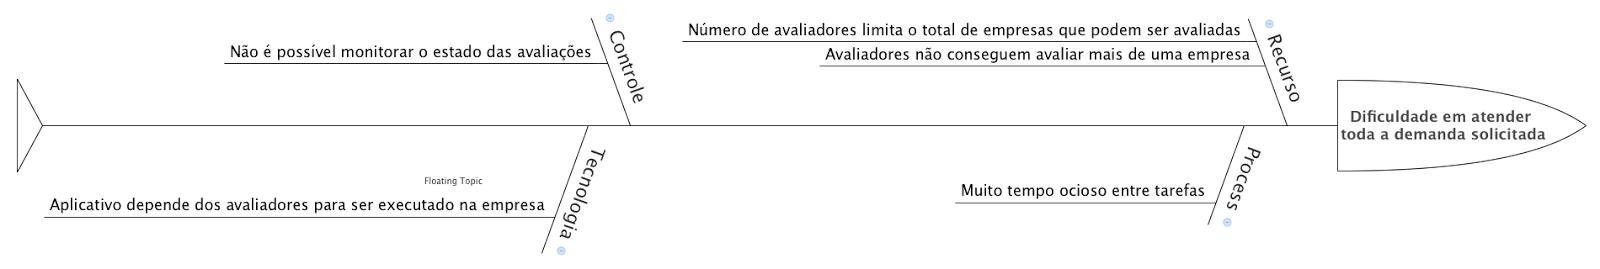
\includegraphics[scale=0.55]{fishbone}
		\caption[Diagrama de Fishbone]{Diagrama de Fishbone.}
		\label{fig:fishbone}
	\end{figure}
	\vspace*{\fill}
\end{landscape}

	\section[Processo a ser Melhorado]{Processo a ser Melhorado}
	\label{sec:contexto_problema}
		Anteriormente, no primeiro relatório do grupo de MPR, foi definido que o processo priorizado seria o processo de inscrição no MOA. A seguir será apresentada um breve resumo desse processo com o objetivo de contextualizar essa parte do projeto:

\subsection[Inscrição no MOA]{Inscrição no MOA}
\label{subsec:contexto_processoMelhorar_inscricaoMOA}
	\begin{itemize}
	\item{\textbf{Definição}: Permitir que empresas envolvidas no contexto adotado pelo MOA possam solicitar participação e consequentemente serem inscritas, caso sejam autorizadas;}
	\item{\textbf{Responsável}: CHAMEX;}
	\item{\textbf{Outros Participantes}: Empresa que deseja solicitar participação;}
	\item{\textbf{Atividades identificadas no AS-IS}:
		\begin{itemize}
			\item{\textbf{Definir Agenda do MOA}: Criar uma agenda com datas a serem cumpridas;}
			\item{\textbf{Disponibilizar Edital de Participação do MOA}: Disponibilizar edital com informações sobre o MOA;}
			\item{\textbf{Preencher Participação de Solicitação MOA}: Preencher solicitação disponibilizada pela Chamex para que seja possível participar do MOA;}
			\item{\textbf{Avaliação das Solicitações}: Identificar possíveis erros nas solicitações preenchidas pelas empresas como dados inconsistentes ou que estejam faltando;}
			\item{\textbf{Enviar Mensagem de Erro de Preenchimento}: Informar à empresa via e-mail participante quais os erros contidos no preenchimento da solicitação feita por ela;}
			\item{\textbf{Receber Mensagem de Erro de Preenchimento}: Receber via e-mail sobre os erros identificados no preenchimento da solicitação de participação no MOA;}
			\item{\textbf{Analisar Viabilidade de Participação}: Analisar se a empresa que solicitou participação no MOA está contida no contexto elaborado pela Chamex e consequentemente se ela poderá participar do MOA;}
			\item{\textbf{Enviar Resposta para a Empresa}: Informar à empresa via e-mail se ela foi autorizada a participar do MOA;}
			\item{\textbf{Receber Resposta Sobre a Viabilidade}: Receber via e-mail a resposta sobre a adesão no MOA.}
		\end{itemize}}
\end{itemize}
\begin{landscape}
	\vspace*{\fill}
	\begin{figure}[H]
		\centering
		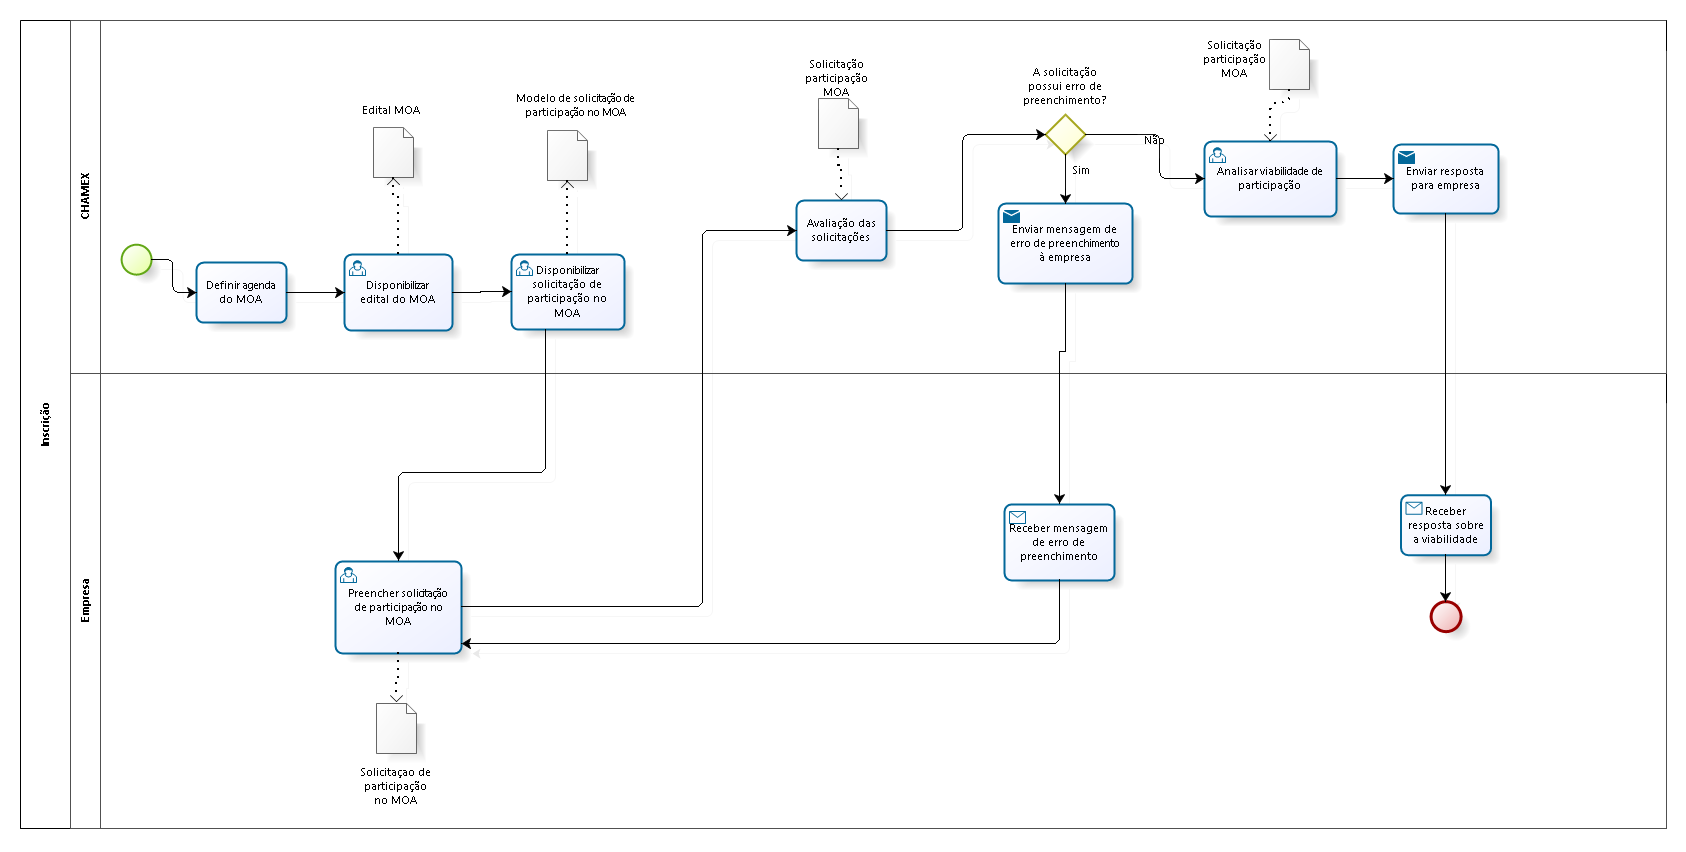
\includegraphics[scale=0.55]{inscricao_moa}
		\caption[Processo de Inscrição no MOA]{Processo de Inscrição no MOA.}
		\label{fig:processo_inscricao}
	\end{figure}
	\vspace*{\fill}
\end{landscape}

	\subsubsection[5W2H]{5W2H}
	\label{subsubsec:contexto_processoMelhorar_inscricaoMOA_5w2h}
		O 5W2H representa um conjunto de perguntas sobre um determinado processo ou atividade que procuram explicar com o máximo de clareza possível o entendimento dos colaboradores da empresa quanto ao assunto. Através das respostas extraídas nessa técnica, é possível adquirir o conhecimento necessário para criar um plano de ação que irá promover a mudança \cite{paim}.
\\ \indent O 5W representa as perguntas \emph{What?}, o que será feito; \emph{Who?}, quem irá fazer; \emph{Where?}, onde será feito; \emph{When?}, quando será feito; \emph{Why?}, porque será feito, tentando responder qual a importância daquilo para a empresa.
\\ \indent O 2H representa as perguntas \emph{How?}, como será feito; \emph{How Much?}, qual o custo relativo.

\begin{table}[H]
	\centering
	\begin{tabular}{|c|p{10cm}|}
		\hline
		\textbf{\emph{What?} O que?} & Inscrição MOA \\ \hline
		\textbf{\emph{Who?} Quem?} & CHAMEX e empresa interessada \\ \hline
		\textbf{\emph{Where?} Onde?} & Empresa CHAMEX e site CHAMEX \\ \hline
		\textbf{\emph{When?} Quando?} & Inicio do período de inscrição \\ \hline
		\textbf{\emph{Why?} Por quê?} & Passo inicial necessário para saber quais empresas vão participar do MOA \\ \hline
		\textbf{\emph{How?} Como?} & Empresas se inscrevem no MOA a partir de uma planilha disponibilizada no site da CHAMEX \\ \hline
		\textbf{\emph{How Much?} Quanto?} & - \\ \hline
	\end{tabular}
	\label{tab:5w2h}
	\caption[5W2H no Contexto de Inscrição no MOA]{5W2H no Contexto de Inscrição no MOA.}
\end{table}

	\section[Simulação AS-IS]{Simulação AS-IS}
	\label{sec:contexto_asis}
		Para a simulação dos processos foi escolhido o processo mais viável a ser tratado da lista de processos da CHAMEX, e também os dois processos de maior valor numérico de prioridade da mesma. Assim será simulado os processos de Inscrição no MOA (mais viável). O tempo de execução e o número de cada tarefa foi baseado no \emph{feedback} do cliente e em casos onde não foi possível haver o conhecimento de tal, foram estimados os dados de acordo com o consenso da equipe de modelagem do processo.
\\ A seguir serão listadas as configurações e resultados para os cenários de simulação.

\subsection[Propriedades dos Cenários de Simulação]{Propriedades dos Cenários de Simulação}
\label{subsec:contexto_asis_cenarios}
	\begin{itemize}
	\item{\textbf{Cenário 1}:
		\begin{itemize}
			\item{\textbf{Duração}: 30 Dias;}
			\item{\textbf{Unidade Básica de Medida}: Horas;}
			\item{\textbf{Instâncias Iniciadas}: 10.}
		\end{itemize}}
	\item{\textbf{Cenário 2}:
		\begin{itemize}
			\item{\textbf{Duração}: 30 Dias;}
			\item{\textbf{Unidade Básica de Medida}: Horas;}
			\item{\textbf{Instâncias Iniciadas}: 30.}
		\end{itemize}}
	\item{\textbf{Recursos Disponíveis}:
		\begin{itemize}
			\item{\textbf{Gerente}: 1;}
			\item{\textbf{Avaliador}: 5;}
			\item{\textbf{Empresa}: 10;}
		\end{itemize}}
\end{itemize}

\subsection[Recursos e Tempo de Processamento do Cenário de Simulação]{Recursos e Tempo de Processamento do Cenário de Simulação}
\label{subsec:contexto_asis_tempo}
	\begin{table}[H]
	\centering
	\begin{tabular}{|p{5cm}|c|c|c|}
		\hline
		\textbf{Atividade} & \textbf{Recurso} & \textbf{Quantidade} & \textbf{Horas} \\ \hline
		Analisar viabilidade de participação & Analista & 1 & 4 \\ \hline
		Avaliação das solicitações & Analista & 1 & 4 \\ \hline
		Definir agenda do MOA & Gerente & 1 & 24 \\ \hline
		Disponibilizar solicitação de participação no MOA & Gerente & 1 & 1.16 \\ \hline
		Disponibilizar edital do MOA & Gerente & 1 & 8 \\ \hline
		Enviar mensagem de erro de preenchimento à empresa & Analista & 1 & 0.5 \\ \hline
		Enviar resposta para empresa & Analista & 1 & 0.5 \\ \hline
		Preencher solicitação de participação no MOA & Empresa & 1 & 48 \\ \hline
		Receber mensagem de erro de preenchimento & Empresa & 1 & 0.16 \\ \hline
		Receber resposta sobre a viabilidade & Empresa & 1 & 0.16 \\ \hline
	\end{tabular}
	\caption[Recursos e Tempo de Processamento do Cenário de Simulação]{Recursos e Tempo de Processamento do Cenário de Simulação}
\end{table}

\subsection[Resultado da Simulação]{Resultado da Simulação}
\label{subsec:contexto_asis_resultado}
	O tempo total médio do processo foi de 231.17 horas para o cenário 1 e 627.83 horas para o 2. A Figura \ref{fig:resultadosasis} apresenta os resultados da simulação.
\begin{figure}[H]
	\centering
	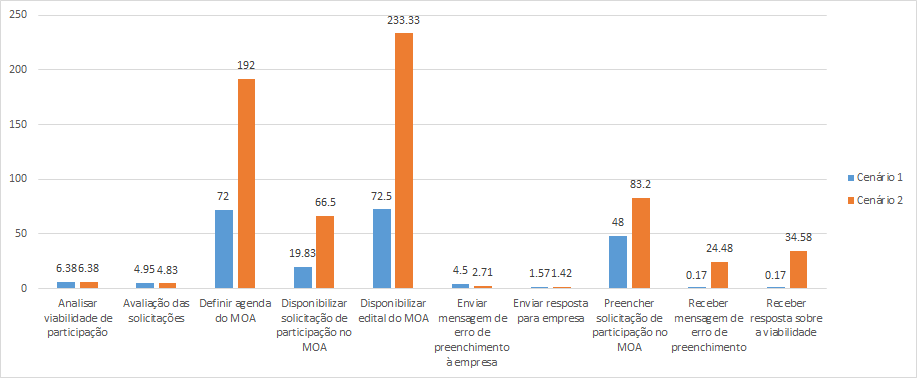
\includegraphics[scale=0.66]{resultado_asis_simulacao}
	\caption[Gráfico de Resultados da Simulação AS-IS]{Gráfico de Resultados da Simulação AS-IS.}
	\label{fig:resultadosasis}
\end{figure}

\subsection[Recursos]{Recursos}
\label{subsec:contexto_asis_recursos}
	\begin{figure}[H]
	\centering
	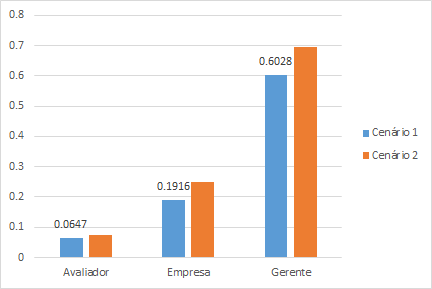
\includegraphics[scale=1]{recursos_asis_simulacao}
	\caption[Gráfico de Recursos da Simulação AS-IS]{Gráfico de Recursos da Simulação AS-IS.}
	\label{fig:recursosasis}
\end{figure}

\subsection[Análise do Resultado]{Análise do Resultado}
\label{subsec:contexto_asis_analise}
	Para ambos os cenários as atividade Definir Agenda do MOA, Disponibilizar Solicitação de Participação no MOA e Disponibilizar Edital do MOA apresentaram um valor mais elevado quanto a média de horas das demais atividades, isso resultou no alto valor para utilização do Gerente no processo.
\\ \indent As demais atividades apresentaram valores próximos do esperado no Cenário 1. No Cenário 2 o tempo foi discrepante devido ao gargalo gerado pelas atividades iniciais do gerente, que acabam influenciando todas as demais. A baixa utilização do analista se mostra preocupante, pois se espera que ele utilize mais o tempo do processo avaliando as solicitações.
	%[MPR]	Identificar pontos de automatização e melhoria do processo;
		%\input{source/}
	%[RS]	De acordo com a estratégia a ser utilizada pelo grupo: identificar e descrever o problema, as necessidades, as características, casos de uso, users stories, temas de investimento, épicos, requisitos funcionais e requisitos não funcionais;
		%\input{source/}
	%[RS]	Aplicar ao menos duas técnicas de elicitação de requisitos;
		%\input{source/}
	%[MPR]	Realizar simulação (TO-BE) e apresentar os resultados;
		%\input{source/}
	%[RS]	Detalhar user stories / casos de uso (referentes à primeira iteração do projeto);
		%\input{source/}
	%[RS]	Registrar os requisitos e a rastreabilidade, proposta no PGR, na ferramenta selecionada;
		%\input{source/}
	%[MPR]	Automatizar o processo redesenhado;
		%\input{source/}
	%[MPR]	Apresentar as melhorias;
		%\input{source/}
	%[MPR]	Apresentar comparação e análise entre o processo redesenhado e o processo “atual”;
		%\input{source/}
	%[MPR]	Definir Metas e indicadores para os processos;
		%\input{source/}
	%[MPR & RS]	Realizar relato de experiência (texto livre), sobre a realização do trabalho;
		%\input{source/}
	%[MPR & RS]	Lições aprendidas
		%\input{source/}
	%[MPR & RS]	Avaliação
		%\input{source/}
	%[MPR & RS]	Planejamento (Cronograma)
		%\input{source/}
	%[MPR]	Apresentar a solução de software, referente à automação do processo, sob a perspectiva de modelagem de processos
		%\input{source/}
	%[RS]	Apresentar a solução de software, referente à automação do processo, sob a perspectiva da engenharia de requisitos
		%\input{source/}

		\bibliography{bibliografia}
		
	\backmatter
		\bookmarksetup{startatroot} 
		\postextual
    		\printindex

\end{document}
